% id: 0350
% book: RPM 중3-2 수학 · 03 원과 직선
% section: 중단원 마무리하기
% figure: crop:fig-0350.png
% answer: ③
% answer_source: 답지
% variant_level: 0 (원본 전사)
% 이 파일은 build.mjs 가 items.json 에서 만든다. 고칠 때는 items.json 을 고친다.
\dmkichul{RPM 중3-2 수학 0350번 · 58쪽 · 중요}
\noindent\begin{minipage}[t]{0.58\linewidth}\vspace{0pt}\raggedright 오른쪽 그림과 같이 $\seg{AD}\parallel\seg{BC}$인 등변사다리꼴~$\pt{ABCD}$가 원~$\pt{O}$에 외접한다. $\seg{AD}=6\,\mathrm{cm}$, $\seg{BC}=10\,\mathrm{cm}$일 때, 원~$\pt{O}$의 둘레의 길이는?\end{minipage}\hfill\begin{minipage}[t]{0.4\linewidth}\vspace{0pt}\centering 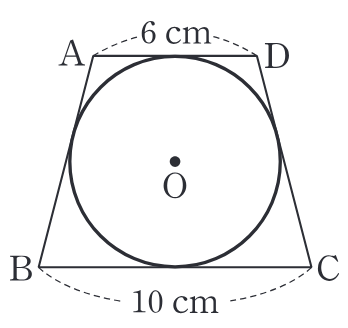
\includegraphics[width=83.5pt]{figures/fig-0350.png}\end{minipage}\par
\begin{choicesii}{\rule[-3ex]{0pt}{8ex}$\sqrt{15}\pi\,\mathrm{cm}$}{\rule[-3ex]{0pt}{8ex}$4\sqrt{3}\pi\,\mathrm{cm}$}{\rule[-3ex]{0pt}{8ex}$2\sqrt{15}\pi\,\mathrm{cm}$}{\rule[-3ex]{0pt}{8ex}$12\pi\,\mathrm{cm}$}{\rule[-3ex]{0pt}{8ex}$15\pi\,\mathrm{cm}$}\end{choicesii}
